\documentclass[a4paper,12pt]{article}

\usepackage[14pt]{extsizes}
\usepackage{cmap}					% поиск в PDF
\usepackage{mathtext} 				% русские буквы в формулах
\usepackage[T2A]{fontenc}			% кодировка
\usepackage[utf8]{inputenc}			% кодировка исходного текста
\usepackage[english,russian]{babel}	% локализация и переносы
\usepackage{graphicx}
\usepackage{geometry}
\usepackage{amsmath}
\usepackage{amssymb}
\usepackage[table]{xcolor}
\setlength\extrarowheight{2pt}


\geometry{verbose, a4paper, tmargin=2cm, bmargin=2cm, lmargin=3cm, rmargin=2cm}
\author{Vysotsky Maxim}
\title{Отчёт}
\date{2022}

\begin{document}
	\begin{titlepage}
		\begin{center}
			{Министерство науки и высшего образования Российской Федерации
				НОВОСИБИРСКИЙ НАЦИОНАЛЬНЫЙ ИССЛЕДОВАТЕЛЬСКИЙ
				ГОСУДАРСТВЕННЫЙ УНИВЕРСИТЕТ (НГУ)}
		\end{center}
		\begin{center}
			{Физический факультет}
		\end{center}
		\begin{center}
			{Кафедра общей физики}
		\end{center}
		
		
		\vspace{7cm}
		{
			\begin{center}
				{\bf Лабораторная работа №2.2}\\
				Основы измерений в цепях переменного тока
			\end{center}
		}
		\vspace{2cm}
		\begin{flushright}
			{Руководитель:\\ Старший преподаватель\\
				Яцких А. А.\\
				Работу выполнил:\\
				Высоцкий М. Ю.\\
				\vspace{0.2cm}
				гр. 24301}
		\end{flushright}
		\vspace{3cm}
		\begin{center}
			Новосибирск, 2024
		\end{center}
	\end{titlepage}

\section{Теоретическое введение}
\textbf{Цель работы:} Познакомиться с принципом действия цифровых измерительных приборов; научиться проводить измерения в цепях переменного тока, определить рабочий диапазон по частоте различных цифровых мультиметров, провести измерение величины напряжения сигналов сложной формы и определить режимы работы источника гармонических сигналов.

\textbf{Оборудование:} цифровые мультиметры GDM-8145, осциллограф \\Tektronix, макет с
диодом Д и сопротивлением R, разветвитель – тройник, мультиметр DT838, генератор GFG 8255,  магазин сопротивлений Р33.

\subsection{Задание 1. Изучение влияния частоты измеряемого сигнала на показания вольтметров}
\textbf{Цель задания.} В данном задании требуется снять амплитудно-частотную характеристику - зависимость показаний приборов (в нашем случае мультиметры GDM-8145, DT838) от изменения частоты для гармонического сигнала (синус). По итогу должен получиться график, на котором мы сможем увидеть диапазоны частоты, при которых данное оборудование показывает неверные значения напряжения (и, наоборот, верные), снятые с генератора (GFG 8255). 

\begin{figure}[h!]
	\begin{center}
		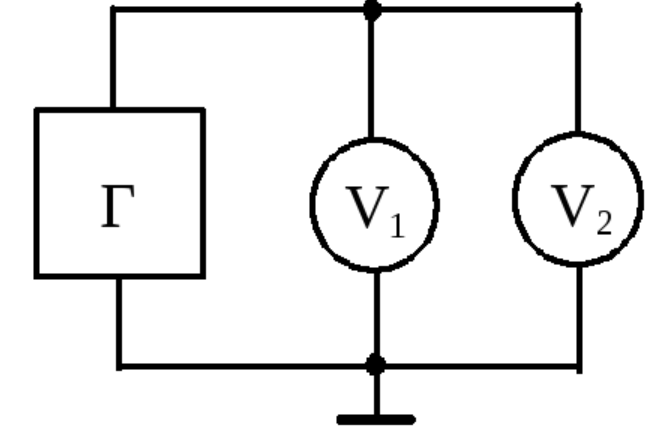
\includegraphics[scale=0.4]{scheme_1.png}
	\end{center}
	\caption{Электрическая схема задания 1.}

\end{figure}


\begin{table}[!ht]
    \centering
    \begin{tabular}{|l|l|l|}
    \hline
        \nu, Гц & U_{GDM}\pm\Delta U_{GDM}, В & U_{DT}\pm\Delta U_{DT}, В\\ \hline
        5,5819 & $6,958\pm0,006$ & $6,3\pm 0,2$ \\ \hline
        5,8577 & $6,989\pm0,006$ & $6,5\pm 0,2$\\ \hline
        6,1448 & $6,972\pm0,006$ & $6,6\pm 0,2$ \\ \hline
        6,6875 & $6,940\pm0,006$ & $6,8\pm 0,2$ \\ \hline
        18,542 & $7,507\pm0,006$ & $7,4\pm 0,2$ \\ \hline
        52,750 & $7,513\pm0,006$ & $7,5\pm 0,2$\\ \hline
        100,90 & $7,514\pm0,006$ & $7,5\pm 0,2$ \\ \hline
        677,71 & $7,527\pm0,006$ & $7,5\pm 0,2$\\ \hline
        302,81 & $7,490\pm0,006$ & $7,4\pm 0,2$ \\ \hline
        22013 & $7,518\pm0,006$ & $7,4\pm 0,2$ \\ \hline
        49009 & $7,480\pm0,006$ & $7,2\pm 0,2$ \\ \hline
        11065 & $7,539\pm0,006$ & $6,7\pm 0,2 $\\ \hline
        26838 & $7,555\pm0,006$ & $5,5\pm 0,2$ \\ \hline
        40670 & $7,608\pm0,006$ &$ 4,8\pm 0,2 $\\ \hline
        50061 & $7,519\pm0,006$ & $4,4\pm 0,2$ \\ \hline
        53501 & $7,472\pm0,006$ & $4,2 \pm 0,2 $\\ \hline
        61626 & $7,435\pm0,006$ & $4,1\pm 0,2$ \\ \hline
        74549 & $7,102\pm0,006 $& $3,7\pm 0,2 $\\ \hline
        125310 &$ 4,644\pm0,005$ & $2,7\pm 0,2$ \\ \hline
        169120 &$ 2,954\pm0,005$ & $2,1\pm 0,2$ \\ \hline
        250420 & $1,288\pm0,004$ &$ 1,6\pm 0,2$ \\ \hline
        237560 & $1,523\pm0,004$ & $1,6\pm 0,2 $\\ \hline
        496570 & $0,050\pm0,004$ & $1,1\pm 0,2$ \\ \hline
        407690 & $0,228\pm0,004$ & $1,0\pm 0,2$ \\ \hline
        529520 & $0,020\pm0,004$ & $1,0\pm 0,2$ \\ \hline
        1076200 & $0,035\pm0,004$ &$ 0,1\pm 0,2$ \\ \hline
        2286800 & $0,273\pm0,004$ &$ 4,4\pm 0,2$ \\ \hline
        4046000 & $0,205\pm0,004$ & $-10,6\pm 0,2$ \\ \hline
        5036200 & $0,174\pm0,004$ & $-10,6\pm 0,2$ \\ \hline
    \end{tabular}
    \caption{Результаты эксперимента, задание 1}
\end{table}

\newpage

Далее будут приведены графики амплитудно-частотных характеристик для обоих мультиметров.
\begin{figure}[h!]
	\begin{center}
		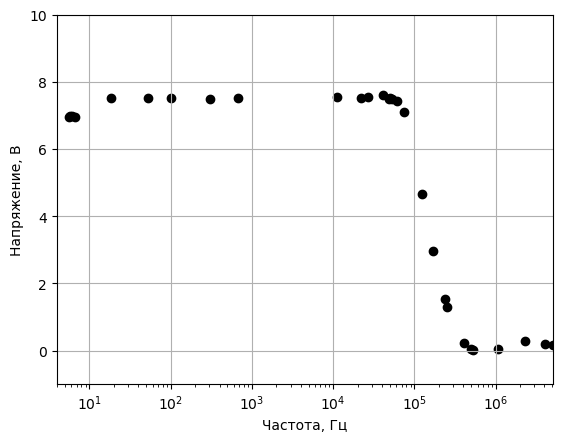
\includegraphics[scale=0.55]{1.png}
	\end{center}
	\caption{Зависимость напряжения на GDM-8145 от частоты.}
\end{figure}

\begin{figure}[h!]
	\begin{center}
		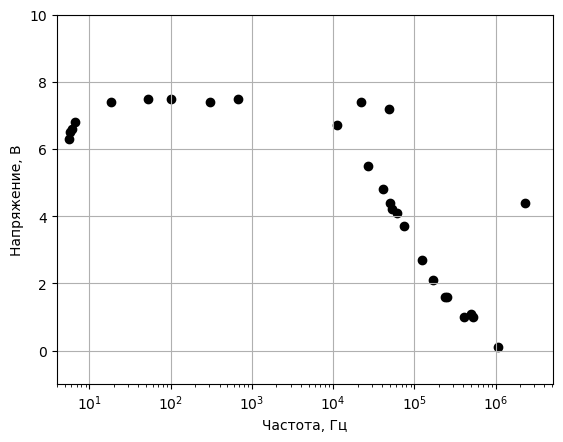
\includegraphics[scale=0.55]{2.png}
	\end{center}
	\caption{Зависимость напряжения на DT838 от частоты.}
\end{figure}

\vspace{2cm}

\subsection{Вывод по заданию}
\hspace{\parindent}Как видно из графиков и полученных значений, в области около 7 Гц оба мультиметра показывают заведомо неверные значения. Параллельно к цепи был подключён осциллограф, показания которого находились в интервале от 7,58 до 7,59 Гц. 

Из внешнего вида графика видно, что с нарастанием частоты показание напряжению стремилось к истинному значению, и спустя какое-то время, в различных точках для каждого из мультиметров оно вновь становилось меньше.

Основываясь на полученных данных, для мультиметра GDM-8145 левой границей предлагается выбрать показание приблизительно в 7 Гц, а правой - 53 кГц. В промежутке между ними показания мультиметра приближены к реальным. Для мультиметра DT838 левой границей предлагаю выбрать также 7 Гц, а правой - 22 кГц.

К сожалению, данных недостаточно для определния чёткого момента перегиба графика зависимости и предъявления более конкретных чисел. Ошибки объясняются не совсем точной методикой выполнения задания, так как при первой серии измерений изначально бралось слишком много точек, а во второй серии бралось слишком мало промежуточных значений (что хорошо видно по графикам на промежутке от $10^3$ до $10^4$ Гц). Однако этих показаний достаточно, чтобы сделать вывод о пропускной линии обоих мультиметров.

По паспорту GDM имеет пропускную линию от 20 Гц до 50 кГц. Таким образом можно сказать, что экспериментальные данные попадают в интервал для мультиметра GDM-8145. По крайней мере, полученные показатели близки к паспортным. 

Однако для мультиметра DT838 мне найти таких данных в паспорте, увы, не удалось \textit{(или я плохо читал...)}

Нетрудно заметить, что мультиметр DT838 $"сдаётся"$ на более низких частотах, чем GDM-8145, что может быть объяснено его дешевизной и, соответственно, простым устройством самого прибора. К тому же нужно учитывать разного рода помехи (и тут мы опускаем их перечисление в силу их неизученности), шумы и другие внешние факторы.


\subsection{Задание 2. Измерение напряжения периодических сигналов без постоянной составляющей}
\textbf{Цель задания.} В данном задании требуется измерить амплитуду синусоидального, треугольного и прямоугольного сигналов, а также проверить
истинность теоретически выведенных зависимостей амплитудного и эффективного
напряжения.

\newpage
Схема установки приведена ниже.
\begin{figure}[h]
	\begin{center}
		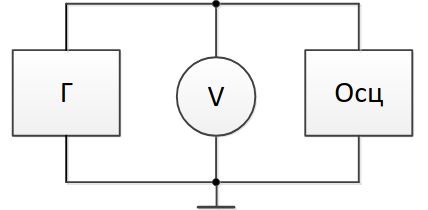
\includegraphics[scale=0.55]{scheme_2.png}
	\end{center}
	\caption{Электрическая схема, задание 2}
\end{figure}


Результаты эксперимента.
\begin{table}[!ht]
    \centering
    \begin{tabular}{|l|l|l|l|l|l|}
    \hline
        Частота, Гц & U_{GDM}\pm\Delta, В & U_{Pk}\pm\Delta, В & U_{0}\pm \Delta U_{0}, В & U_{RMS}\pm\Delta, В &  \\ \hline
        1,0088 & 3,369\pm 0,048 & 9,84\pm 0,30 & 4,92\pm 0,30 & 3,48\pm 0,15 & sin\\ \hline
        1,0086 & 2,878\pm 0,043 & 10,0\pm 0,30 & 5,00\pm 0,30 & 2,89\pm 0,15 & \Delta \\ \hline
        1,0086 & 5,254\pm 0,067 & 10,7\pm 0,32 & 5,35\pm 0,32 & 5,25\pm 0,16 & \[\Box\] \\ \hline
    \end{tabular}
    \caption{Результаты эксперимента, задание 2}
\end{table}


Для поиска значений $U$ использовались следующие выражения для эффективного напряжения гармонического сигнала:

\begin{equation}\label{sinus}
    sin: U_{RMS} = \sqrt{\frac{2}{T} \int\limits_0^{T/2} U_0^2\sin(\omega t)dt} = \frac{U_0}{\sqrt{2}}
\end{equation}

\begin{equation}\label{triagle}
    \Delta: U_{RMS} = \sqrt{\frac{4}{T} \int\limits_0^{T/4} (4t/T)^2dt} = \frac{U_0}{\sqrt{3}}
\end{equation}

\begin{equation}\label{kvadr}
    \Box: U_{RMS} = \sqrt{\frac{2}{T} \int\limits_0^{T/2} U_0^2dt} = U_0
\end{equation}

\newpage
\subsection{Вывод по заданию}

\hspace{\parindent}Исходя из данных таблицы, показания напряжения на осциллографе и мультиметре лежат в пределах погрешностей, следовательно, приборы показывают приблизительно одинаковые значения. Откуда мы можем говорить о справедливости формул (\ref{sinus}), (\ref{triagle}) и (\ref{kvadr})
Однако нужно отметить, что мультиметр показывает \textbf{больше знаков после запятой}. Потому мультиметр будет предпочтительнее для измерения небольших напряжений, нежели осциллограф.


\subsection{Задание 3}
\textbf{Цель задания.} В этом задании нужно снять показания осциллографа и мультиметра (в режиме DC и AC) и вычислить амплитудное значение напряжения. Также нужно сравнить его с амплитудой, измеренной осциллографом.

\begin{figure}[h]
	\begin{center}
		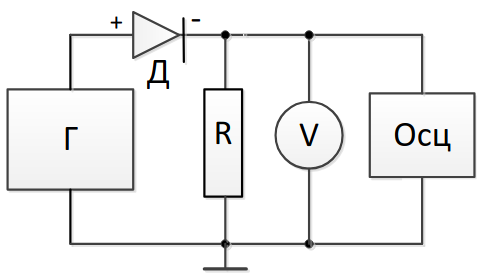
\includegraphics[scale=0.4]{scheme_3.png}
	\end{center}
	\caption{Электрическая схема, задание 3}.
\end{figure}

Ниже приведены данные, снятые в ходе работы.

\begin{table}[ht!]
    \begin{tabular}{|l|l|l|l|l|l|l|l|}
    \hline
        \nu, Гц & Режим & & U_0\pm\Delta, В & U_{ср}\pm\Delta, В & U_{RMS}\pm\Delta, В & U_{GDM}\pm\Delta, В \\ \hline
        100,19 & DC & sin & 10,2\pm0,3 & 5,1\pm0,3 & 3,2\pm0,3  &3,105\pm0,030 \\ \hline
        100,16 & AC & sin & 10,2\pm0,3 & 5,1\pm0,3 &  3,2\pm0,3 &4,906\pm0,038  \\ \hline
        100,17 & DC & \Delta & 10,6\pm0,3 & 4,3\pm0,3 & 2,6\pm0,3  &2,522\pm0,027  \\ \hline
        100,17 & AC & \Delta & 10,6\pm0,3 & 4,3\pm0,3 & 2,6\pm0,3  &4,167\pm0,036  \\ \hline
        100,17 & DC & \[\Box\] & 10,6\pm0,3 & 7,5\pm0,3 & 5,3\pm0,3  &5,176\pm0,041   \\ \hline
        100,17 & AC & \[\Box\] & 10,6\pm0,3 & 7,5\pm0,3 & 5,3\pm0,3 &7,326\pm0,050  \\ \hline
    \end{tabular}
    \caption{Результаты эксперимента, задание 3}
\end{table}


Связь между эффективным и амплитудным значением для выражается следующим образом:
\begin{equation}\label{amplit}
    \sin: U_{RMS} = \frac{U_0}{2}
\end{equation}

\begin{equation}
    \Delta: U_{RMS} = \frac{U_0}{\sqrt{6}}
\end{equation}

\begin{equation}
    \Box: U_{RMS} = \frac{U_0}{\sqrt{2}}.
\end{equation}

Связи для среднего и амплитудных значений:

\begin{equation}\label{amplit}
    \sin: U_{ср} = \frac{U_0}{\pi}
\end{equation}

\begin{equation}
    \Delta: U_{ср} = \frac{U_0}{4}
\end{equation}

\begin{equation}
    \Box: U_{ср} = \frac{U_0}{2}.
\end{equation}



\subsection{Вывод по заданию}

\hspace{\parindent}Использовав последние 6 формул мы получим следующие значения напряжения.
\begin{table}[h]
    \centering
    \begin{tabular}{|l|l|l|}
    \hline
        U_0\pm\Delta U_0, В & U\pm\Delta U, В & График\\ \hline
         10,2\pm0,3 &9,754\pm0,030 &sin \\ \hline 
         10,2\pm0,3 &9,812\pm0,038&sin \\ \hline 
         10,6\pm0,3 &10,088\pm0,027 &\Delta \\ \hline 
         10,6\pm0,3 &10,207\pm0,036 &\Delta \\ \hline 
         10,6\pm0,3 &10,352\pm0,041 &\[\Box\] \\ \hline 
         10,6\pm0,3 &10,360\pm0,050 &\[\Box\] \\ \hline 
    \end{tabular}
    \caption{Сравнение показаний мультиметра и осциллографа, задание 3}
\end{table}

Как видно из таблицы, показания лежат в пределах погрешностей, что говорит об истинности формул, а также верности проведённого эксперимента. Учитывая порядок величины и погрешности в GDM можно сделать вывод, что он, действительно, при низких показаниях напряжений даёт более точную картину, нежели осциллограф.

\newpage

\subsection{Задание 4}
\textbf{Цель задания.} Определить оптимальное сопротивление нагрузки, при котором на ней выделяется
максимальная мощность.

\begin{table}[!ht]
    \centering
    \begin{tabular}{|l|l|l|l|l|}
    \hline
        Частота, Гц & R, Ом & U, В & I, мА & P, мВт \\ \hline
        49,893 & 99,9 & $5,076 \pm 0,17$& $50,78 \pm 0,26$& $257,76\pm0,43$ \\ \hline
        49,893 & 94,9 & $4,986 \pm 0,16$& $52,52 \pm 0,27$& $261,86\pm0,44$ \\ \hline
        49,893 & 89,9 &$ 4,892 \pm 0,16$& $54,42 \pm 0,28$& $266,22\pm0,44 $\\ \hline
        49,893 & 84,9 & $4,791 \pm 0,16$& $56,44 \pm 0,29$& $270,40\pm0,45 $\\ \hline
        49,893 & 79,9 & $4,684 \pm 0,16$& $58,59 \pm 0,30$& $274,44\pm0,46$ \\ \hline
        49,893 & 74,9 & $4,567 \pm 0,15$& $60,92 \pm 0,31$& $278,22\pm0,47$ \\ \hline
        49,893 & 69,9 & $4,440 \pm 0,15$& $63,50 \pm 0,33$& $281,94\pm0,48 $\\ \hline
        49,893 & 64,9 & $4,302 \pm 0,14$& $66,27 \pm 0,34$& $285,09\pm0,49 $\\ \hline
        49,893 & 59,4 &$ 4,151 \pm 0,14$& $69,19 \pm 0,36$& $287,21\pm0,50 $\\ \hline
        49,893 & 54,9 & $3,987 \pm 0,13$& $72,51 \pm 0,37$& $289,10\pm0,51 $\\ \hline
        49,893 & 49,9 & $3,804 \pm 0,13$& $76,21 \pm 0,39$& $289,90\pm0,52 $\\ \hline
        49,893 & 44,9 & $3,605 \pm 0,12$& $80,23 \pm 0,41$& $289,23\pm0,53 $\\ \hline
        49,893 & 39,9 & $3,386 \pm 0,12$& $84,97 \pm 0,43$& $287,71\pm0,55$ \\ \hline
        49,893 & 34,9 & $3,168 \pm 0,11$& $89,68 \pm 0,46$& $284,11\pm0,57 $\\ \hline
        49,893 & 29,9 & $2,856 \pm 0,10$& $95,41 \pm 0,49$& $272,49\pm0,59 $\\ \hline
        49,893 & 24,9 &$ 2,538 \pm 0,09$& $101,82 \pm 0,52$& $258,42\pm0,61 $\\ \hline
        49,893 & 19,9 & $2,180 \pm 0,08$& $109,07 \pm 0,56$& $237,77\pm0,64 $\\ \hline
        49,893 & 14,9 & $1,761 \pm 0,07$& $117,52 \pm 0,60$& $206,95\pm0,67 $\\ \hline
        49,893 & 9,9 &$1,264 \pm 0,05$& $127,56 \pm 0,65$& $161,24\pm0,70 $\\ \hline
        49,893 & 4,9 &$ 0,685 \pm 0,04$& $139,24 \pm 0,71$& $95,38\pm0,74 $\\ \hline
    \end{tabular}
\end{table}

Что сохранить порядок погрешностей, было принято решение представить мощность в милливаттах.

\begin{figure}[ht!]
    \centering
    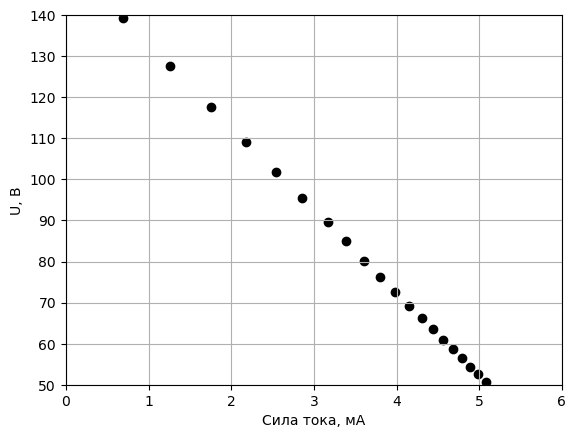
\includegraphics[scale=0.7]{3_2.png}

        \caption{Зависимость I(U)}
\end{figure}

\newpage
\begin{figure}[ht!]
    \centering
    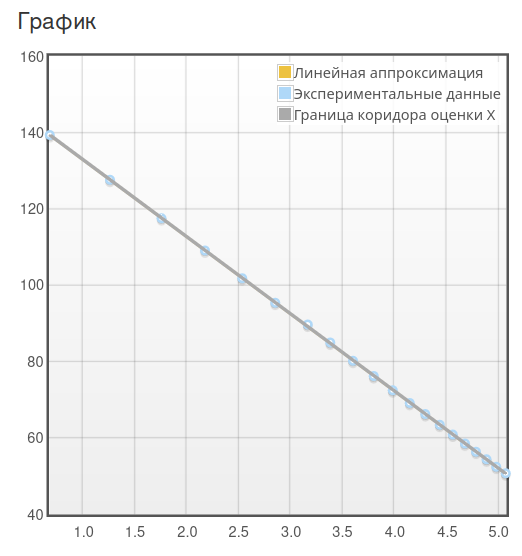
\includegraphics[scale=0.7]{MNK_1.png}
    \caption{График I(U), построенный методом наименьших квадратов}
\end{figure}

\begin{figure}[ht!]
    \centering
    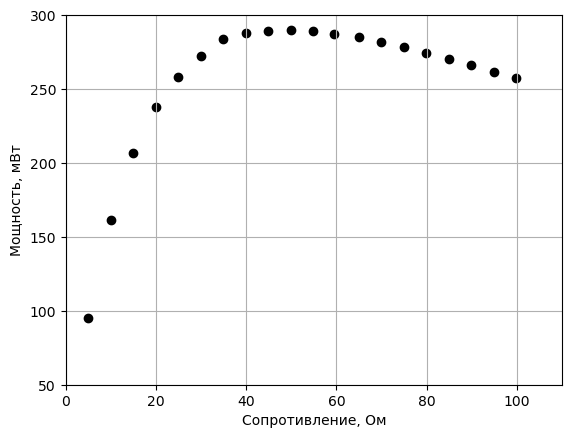
\includegraphics[scale=1]{4_1.png}
    \caption{Зависимость P(R)}
    \label{fig:enter-label}
\end{figure}

\clearpage

\subsection{Вывод по заданию}
\hspace{\parindent}Из первого графика видно, что сила тока падает практически линейно с линейным увеличением напряжения. 

Из графика P(R) можно видеть, что максимальная мощность достигается в значении, близком к сопротивлению источника (на графике 49,9 \approx 50 \hspace{5pt}Ом).



\section{Погрешность измерений}
\hspace{\parindent}В данной работе относительная погрешность представлялась лишь погрешностью самих приборов при снятии напряжений и токов.

Данные брались из паспортов приборов. Нужно отметить, что погрешности зависят от типа тока и напряжения, отчего мы получаем разные порядки погрешностей и точности измерений.

Однако одна погрешность не меняется в течение работы - погрешность осциллографа при определении напряжения составляет 3\%.
\section{Вывод}

В данной работе мною изучено:
\begin{enumerate}
    \item Принцип работы с мультиметром GDM.
    \item Принцип работы с мультиметром DT.
    \item Принцип работы с осциллографом.
    \item Работа с относительной погрешностью, связанной с приборами. Типы разновидности погрешности, зависящей от разного типа тока и напряжения.
    \item Подтверждена истинность всех формул, приведённых в теоретических материалах.
    \item Определена полоса пропускания у мультиметров, определены левая и правая границы для них.
\end{enumerate}
Помимо вышепреведенных выводов нужно отметить, что пришлось вновь изучить \LaTeX, воспользоваться новым программным инструментарием для визуализации данных (Python: Matplotlib)

\centering \textbf{:)}


\end{document}

